\documentclass[10pt]{beamer}
\usepackage{hyperref}
\usepackage{bm}
\usepackage[
    style=authoryear,
    backend=biber
]{biblatex}
\usepackage{caption}
\captionsetup[figure]{labelformat=empty, font=scriptsize}

\usetheme{wur}

\title{Programming for the web}
\subtitle{An introduction to front-end development with React}
\author{Rens Holmer}
\institute{Wageningen University -- Bioinformatics}

\setbeamertemplate{navigation symbols}{}

\begin{document}

\begin{frame}
    \titlepage
\end{frame}

\begin{frame}{Web development in bioinformatics}
    \begin{figure}
        \begin{minipage}{.3\linewidth}
            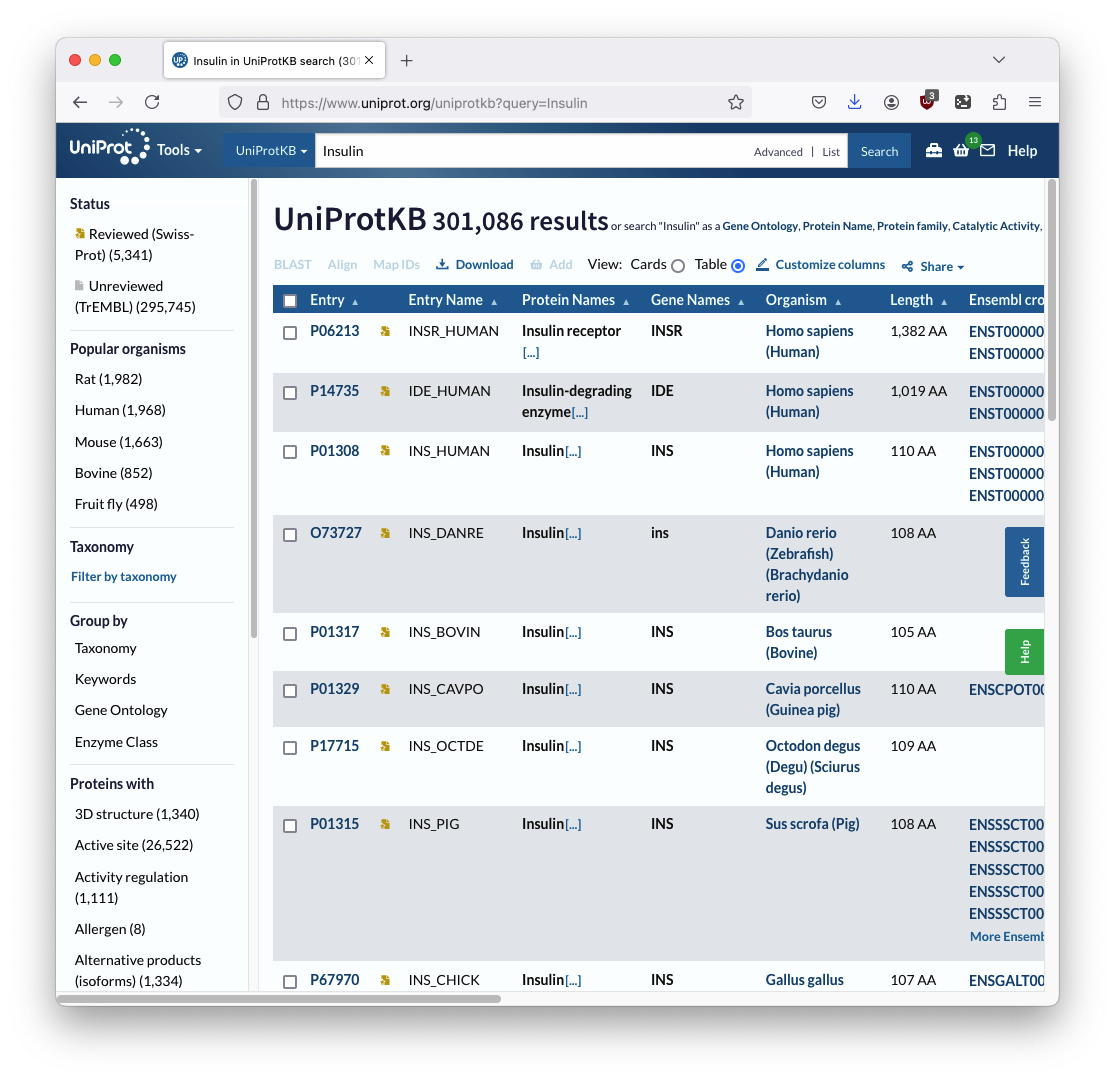
\includegraphics[
                width=\linewidth
            ]{figures/uniprot.png}
            \\ \tiny{Uniprot}
        \end{minipage}
        \begin{minipage}{.3\linewidth}
            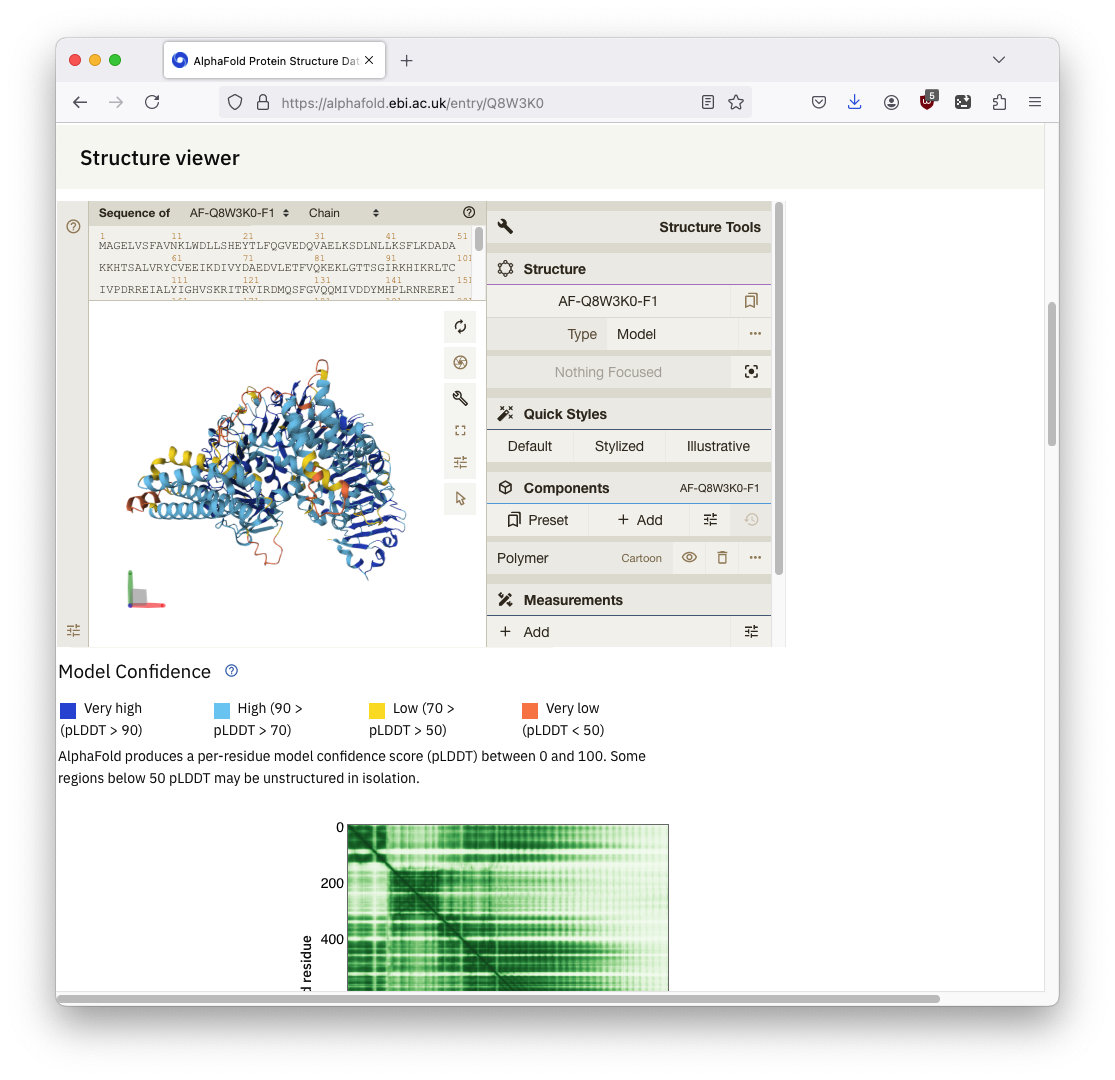
\includegraphics[
                width=\linewidth
            ]{figures/alphafold-db.png}
            \\ \tiny{Alphafold-DB}
        \end{minipage}
    \end{figure}
    \begin{figure}
        \begin{minipage}{.3\linewidth}
            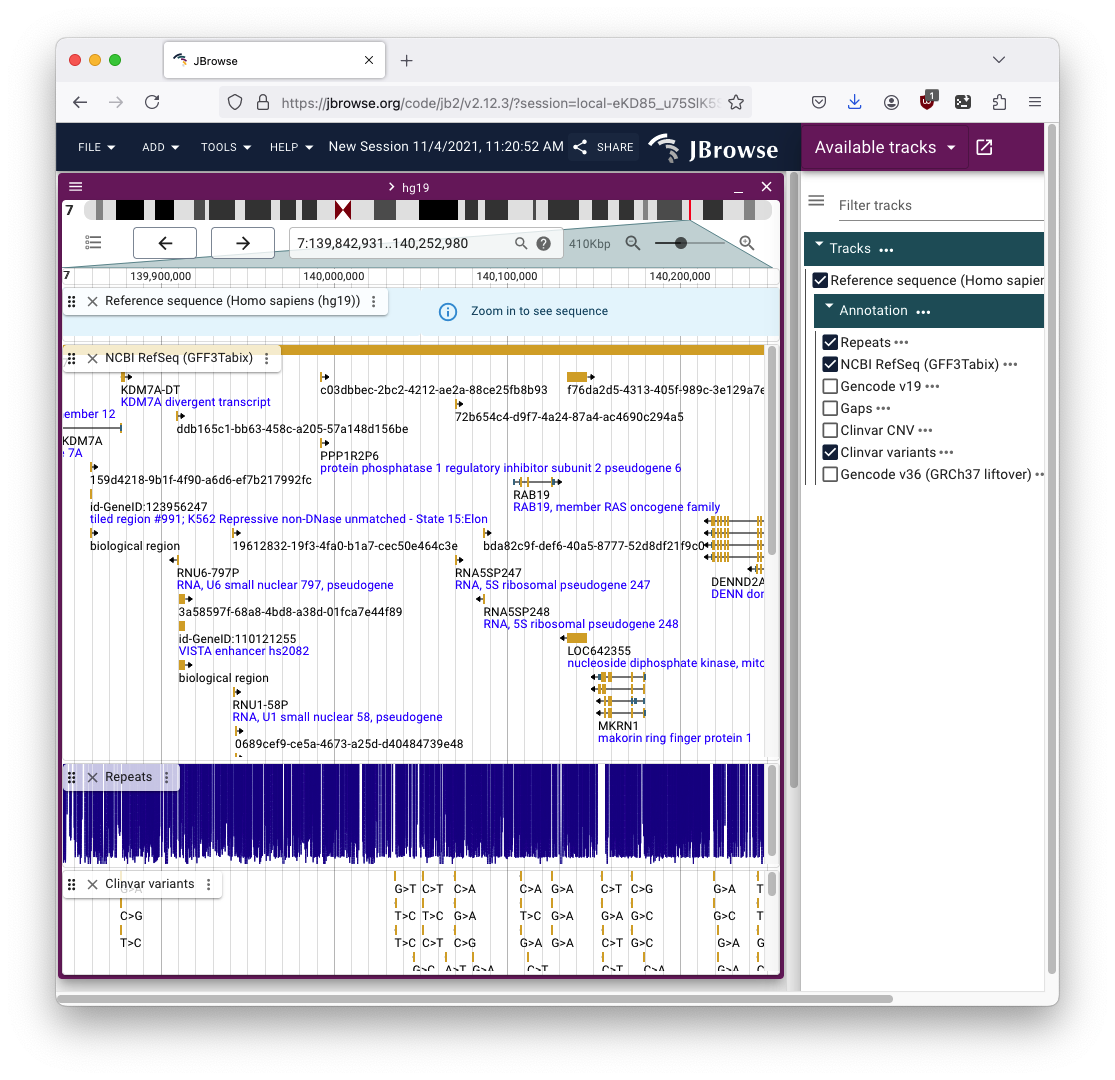
\includegraphics[
                width=\linewidth,
            ]{figures/jbrowse.png}
            \\ \tiny{JBrowse}
        \end{minipage}
        \begin{minipage}{.3\linewidth}
            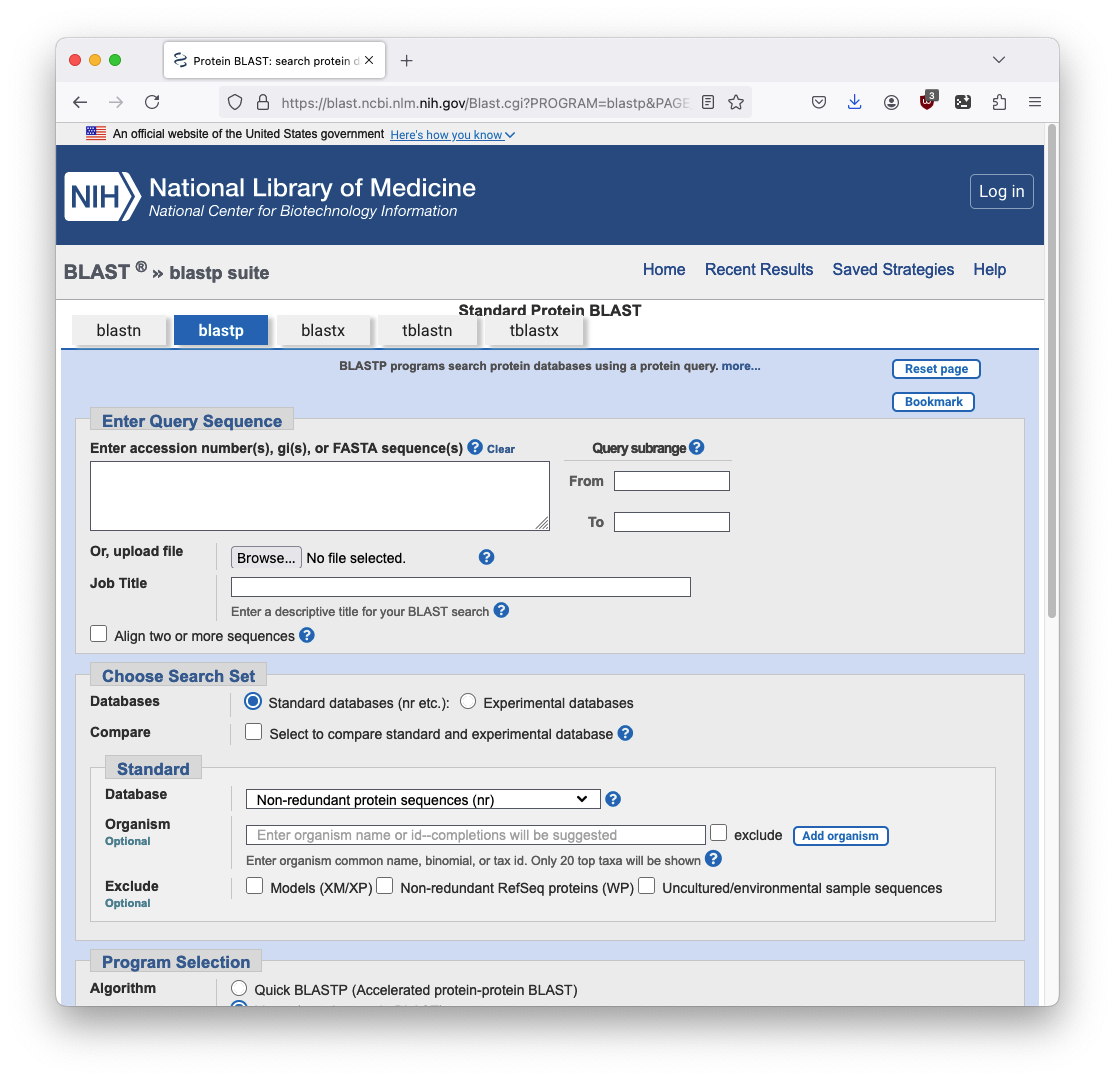
\includegraphics[
                width=\linewidth,
            ]{figures/ncbi-blast.png}
            \\ \tiny{NCBI BLAST}
        \end{minipage}
    \end{figure}
\end{frame}

\begin{frame}

    {\huge Goal of this session}
    \begin{itemize}
        \item Introduction to building \textit{interactive} websites
    \end{itemize}
    \vspace{2em}
    {\large Activities}
    \begin{itemize}
        \item Familiarize yourself with main building blocks of a website
        \item Learn about modern toolchains and frameworks for the web
        \item Build your own interactive bioinformatics data visualization
    \end{itemize}
    \vspace{1em}
    {\large Material}
    \begin{figure}
        
\includegraphics[width=.99\linewidth]{figures/material-link.png}
    \end{figure}
\end{frame}

\begin{frame}

    {\huge Assignment I}

    \vspace{1em}
    Explore two versions of a simple static website:

    \vspace{.5em}

    \texttt{example/simple\_site}

    \texttt{example/simple\_site\_single\_file}


    \vspace{2em}
    \begin{itemize}
        \item Open the workshop folder in an IDE (e.g. VSCode)
        \item Open \texttt{index.html} in a web browser
        \item Click the button
        \item Explore the code
        \item \textit{Discuss}
    \end{itemize}
\end{frame}

\begin{frame}{Some technical background}

\end{frame}

\begin{frame}{Javascript quirks I}
\end{frame}

\begin{frame}{Modern JS}
    \begin{itemize}
        \item frameworks
        \item transpiling
        \item component re-use
        \item state management
        \item AJAX
    \end{itemize}
\end{frame}

\begin{frame}{Assigment II}
    Build a React app for visualizing MSAs
\end{frame}



\end{document}

